\documentclass[12pt,letterpaper]{article}
\usepackage{fullpage}
\usepackage[top=2cm, bottom=4.5cm, left=2.3cm, right=2.3cm]{geometry}
\usepackage{amsmath,amsthm,amsfonts,amssymb,amscd}
\usepackage{lastpage}
\usepackage{enumerate}
\usepackage{fancyhdr}
\usepackage{mathrsfs}
\usepackage{xcolor}
\usepackage{graphicx}
\usepackage{listings}
\usepackage{hyperref}

\hypersetup{%
  colorlinks=true,
  linkcolor=blue,
  linkbordercolor={0 0 1}
}
\usepackage{wrapfig}
\renewcommand\lstlistingname{Algorithm}
\renewcommand\lstlistlistingname{Algorithms}
\def\lstlistingautorefname{Alg.}

\lstdefinestyle{Python}{
    language        = Python,
    frame           = lines, 
    basicstyle      = \footnotesize
}

\setlength{\parindent}{0.0in}
\setlength{\parskip}{0.05in}

% Edit these as appropriate
\newcommand\course{CS 639}

%\pagestyle{fancyplain}
\headheight 35pt
\usepackage{xcolor}
% hyperref link defaults to "blue" (0000ff) as this matches our publisher produced pdf style
\definecolor{xlinkcolor}{cmyk}{1,1,0,0}
\usepackage{hyperref}
\fancypagestyle{firstpage}{
  \chead{\textbf{\Large  Bayesian vs Frequentist Approach \\in Medical Research \\}}
  \rhead{\course \\ \today}
  \lhead{ Harsh Sahu\\Lekshmi Thulasidharan }
  \lfoot{}
  \cfoot{}
  \rfoot{\small\thepage}
  \headsep 3em
}


\usepackage{amsmath}
\PassOptionsToPackage{hyphens}{url}
\fancypagestyle{normal}{
  %\renewcommand{\headrulewidth}{0.5pt}
  \headsep 3em
}

% Set the default page style to 'normal'
%\pagestyle{headings}
%\headsep 2em
%\fancyhead[R]{\rightmark}
%\renewcommand{\subsectionmark}[1]{\markright{#1}}

\pagestyle{headings}
\headsep 2em

%% In response to request from AAS 

\begin{document}
\par
%\thispagestyle{fancy}
\thispagestyle{firstpage}
\section{Introduction}
In medical research, statistical methods are commonly used to analyze data and draw conclusions. Two common approaches are the Bayesian and frequentist approaches. In simple words, Bayesian statistics involves the use of past/existing knowledge (a.k.a prior) along with the new data to make predictions, while frequentist statistics involves making inferences based on the observed data alone. We start this review with a comprehensive overview of each approach followed by a comparison study. Specifically, we try to answer the following questions:
\begin{itemize}
    \item What are the relative strengths and weaknesses of Bayesian and frequentist methods in the context of medical research?
    \item  Under which circumstances do the two approaches lead to similar or different conclusions?
    \item Does the use of one of these approaches increase the potential for breakthroughs in medical research compared to the other?
    \item What are the drawbacks of each approach?
\end{itemize}
We then review the application of Bayesian and frequentist methods in predicting the risk of dementia in older adults. 
\subsection{Frequentist Approach}
explain the foundations

\subsection{Bayesian Approach}
explain the foundations
\subsection{Comparison}
Also talk about medical research application. Case study : Dementia

\section{Application of frequentist approach in risk prediction of dementia in older adults}
Dementia is a common yet severe condition that primarily affects elder population. This is an umbrella term for conditions which could impair a person's ability to perform day to day activities since it has a detrimental effect on their cognition. For example, those who have dementia will experience memory loss, difficulty with communication and reasoning and changes in psychological health. Unfortunately, there is currently no known cure for dementia. For this reason, it is extremely important to identify the individuals who are at very high risk for dementia early on, since this allows for incorporating lifestyle changes and treatments which could potentially slow the rate of progression of this condition. A straightforward method which allows the early identification of risk factors of dementia is by utilising statistical techniques to generate a risk score model. Researchers assign a score to every possible risk factors including demographic factors that could contribute to the development of dementia. Once we have the model, we can screen people and classify them into low, moderate and high risk populations. Within the frequentist approach, one statistical technique that can be highly effective in creating risk prediction models is the``Logistic regression''. Here we review Barnes et al. (2009), where they developed one such risk score model i.e., a late life dementia index which can be used to accurately predict the chances of a person developing dementia in 6 years based on several risk factors using Logistic Regression. The tool they developed can be used to classify individuals into low, moderate and high risk categories for dementia, and hence serves as an excellent tool for monitoring vulnerable adults for dementia symptoms to start their treatment early on.  

\subsection{Logistic Regression}

\begin{wrapfigure}{r}{7cm}
\vspace{-7 mm}
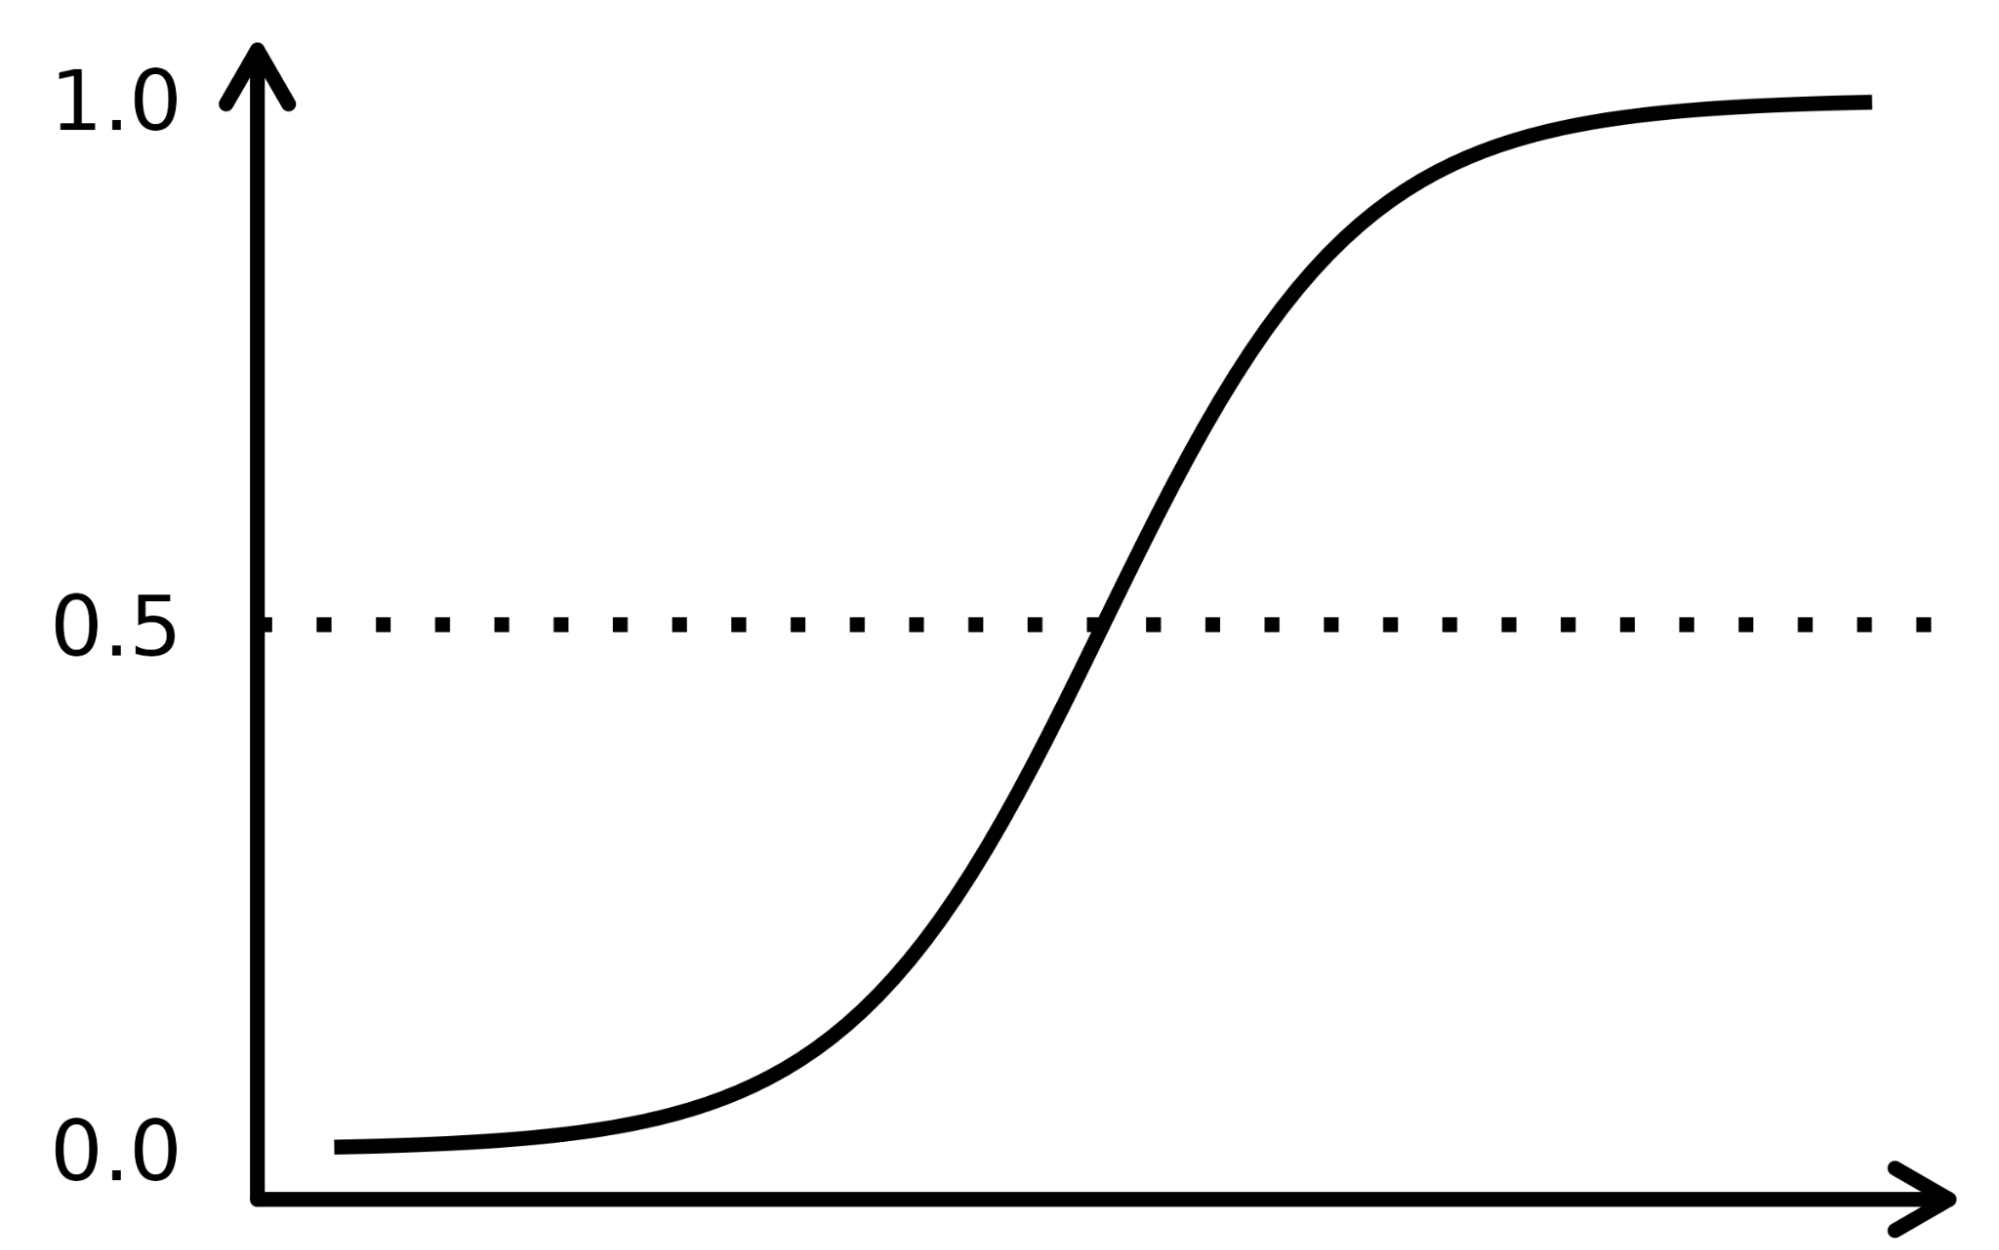
\includegraphics[width=7 cm]{sigmoid.png}
\caption{The sigmoid function curve}
\label{dvdr}
\end{wrapfigure}
Logistic Regression is a useful method for classification problems where we want to find the probability of a variable belongs to a particular category. So, this analysis is best for predicting binary outcomes like yes or no. In medical research this could translate into the probability of a patient developing a disease given one or more input variables (which would be the suspected risk factors). The probability is modelled using a logistic function which is a sigmoid (Fig.\ref{dvdr}) . The function takes a linear combination of the input variables and  and returns an output between 0 and 1. \\

When we have multiple input variables as in the case of risk prediction of a disease, the logistic function takes the form:
\begin{equation}
p(X) =Pr (Y|X)= \frac{e^{\beta_0+\beta_1X_1+\beta_2X_2+...+\beta_pX_p}}{1+e^{\beta_0+\beta_1X_1+\beta_2X_2+...+\beta_pX_p}}
\end{equation}

In the context of the paper we are discussing here, $Pr (Y|X)$ would the probability of a person developing dementia (modelled with variable $Y$) given certain risk factors (or predictors) assumed to be independent with each other($X=(X_1,X_2,\dots,X_p)$). The $\beta$ coefficients represent the parameters of the model, with $\beta_0$ being the intercept and $\beta_1,\beta_2,\dots,\beta_p$ being the coefficients for each of the independent variables. The coefficients can be estimated by maximizing the corresponding likelihood function.  

\subsection{Predictors of Dementia}
The authors considers a wide range of predictors for this study and they belong to several categories. The data for these different risk factors were collected from the Cardiovascular Health Cognition Study which was initiated in 1989 –1990 and updated during 1992–1993. They identified and classified individuals into three groups: (i) Those who already had dementia at the time of data collection, (ii) those who developed dementia after the data collection and (iii) those who developed mild cognitive impairment (less severe than dementia) any time during the follow up period lasted until 1998-1999.








\end{document}
